\input{analysis/template_fitting/figs/template_fit_flow_chart}

This subsection describes template fitting for reaction decomposition.
As mentioned earlier, three possible reactions in the $K^- d \rightarrow n \pi^+ \pi^- n$ final state were mentioned.
Among them, backward $\pi \Sigma$ scattering (Figure \ref{fig:kd_npipin_type}-(a)) and
forward $\pi \Sigma$ production (Figure \ref{fig:kd_npipin_type}-(c)) can be divided into two categories
depending on the charge state of $\pi \Sigma$.
In other words, template events were generated for the following five reactions:

\begin{enumerate}
\item $K^- d \rightarrow n_{forward} \pi^- \Sigma^+$ (Signal-1)
\item $K^- d \rightarrow n_{forward} \pi^+ \Sigma^-$ (Signal-2)
\item $K^- d \rightarrow n K^0 n$ ($K^0$ production)
\item $K^- d \rightarrow \Sigma^+ \pi^- n$ ($\Sigma^+_{forward}$ production)
\item $K^- d \rightarrow \Sigma^- \pi^+ n$ ($\Sigma^-_{forward}$ production)
\end{enumerate}

Among these, reaction 3 is considered an elementary process in which the $K^-$ strikes the proton in the deuteron,
converting it into a neutron that is emitted forward, while the $K^-$ itself recoils backward as a $K^0$.
In this reaction, the remaing nucleon acts as a spectator with Fermi momentum.
The Fermi momentum is simulated using the results of the $d(e, e' p)n$ reaction \cite{d_fermi_ex}.
In reactions 4 and 5, the $\Sigma$ is scattered forward,
and these are also regarded as elementary processes because a large portion of the $K^-$ beam momentum is transferred to the $\Sigma$ and the $\pi$.
Extensive data on such elementary processes have been collected from scattering experiments using hydrogen targets,
and their angular distributions are summarized in \cite{KP_CEX_1GeV}. 

These three reactions are considered the background in this analysis,
and template events need to be generated for backward $\pi\Sigma$ scattering (reactions 1 and 2), which represent the signal.
However, no experimental data are available for these reactions, as they are two-step processes involving a virtual intermediate $\bar{K}$ particle.
Moreover, the fitting to separate the $\pi^-\Sigma^+$ and $\pi^+\Sigma^-$ modes is performed in each bin of the $d(K^-, n)\pi\Sigma$ missing mass.
Additionally, these Monte Carlo samples are also used for acceptance correction, as described in Section \ref{sec:conversion}.
Therefore, the template events were generated assuming a uniform $\pi\Sigma$ mass distribution.
The second-step scattering, $\bar{K}N\rightarrow \pi\Sigma$, was generated isotropically, assuming S-wave dominance of $\Lambda(1405)$.

Template fitting consists of two tasks: background estimation and the separation of the $\pi^- \Sigma^+$ and $\pi^+ \Sigma^-$ modes.
Background estimation is performed using all $K^- d \rightarrow n \pi^+ \pi^- n$ final state events.
In contrast, the separation of the πΣ charged modes is carried out using events from which background contributions
(such as $K^0$ and $Sigma_{forward}$ production) have been removed.
These events are further divided into bins of the $d(K^-, n)\pi\Sigma$ missing mass.
In other words, these two fittings cannot be performed simultaneously, as they use different event samples.
Thus, the fitting procedure is conducted as illustrated in Figure \ref{fig:flow_chart_tempfit}.

First, an initial fit for $\pi^{\mp} \Sigma^{\pm}$ separation is performed without considering the backgraound contributions.
Next, a background fit is conducted to estimate the contribution from $\pi^{\mp} \Sigma^{\pm}$.
Then, a fit for charge mode separation is carried out, taking background leakage into account.
These fitting steps are iterated five times, as the background and $\pi \Sigma$ spectra influence each other.

Since it was found that the background of $K^0$ production includes reactions that are not elementary processes,
a final fit is performed using $K^0$-selected events to separate these contributions.
This step is referred to as "Fitting for $K^0$ production" in Figure \ref{fig:flow_chart_tempfit} and
is described in detail in Appendix \ref{chapter:K0_ana}.
The final spectrum is obtained by performing one last fit for the $\pi^{\mp} \Sigma^{\pm}$ charge mode separation.
In this fitting, the background is removed within a 3$\sigma$,
meaning that the “fitting for $K^0$ production” has almost no effect on the final result.
These so-called template fittings are performed using ROOT’s TFractionFitter,
which is implemented based on “Fitting with Finite Monte Carlo Samples” \cite{temp_fit}.

\begin{frame}{Template fitting to evaluate background}
  \centering
  $d(K^, n \pi^- \pi^+)"n"$ event.
  \begin{tabular}{ccc}
    \begin{minipage}{0.33\hsize}
      \centering
      $\pi^+ \pi^-$ IM\\
      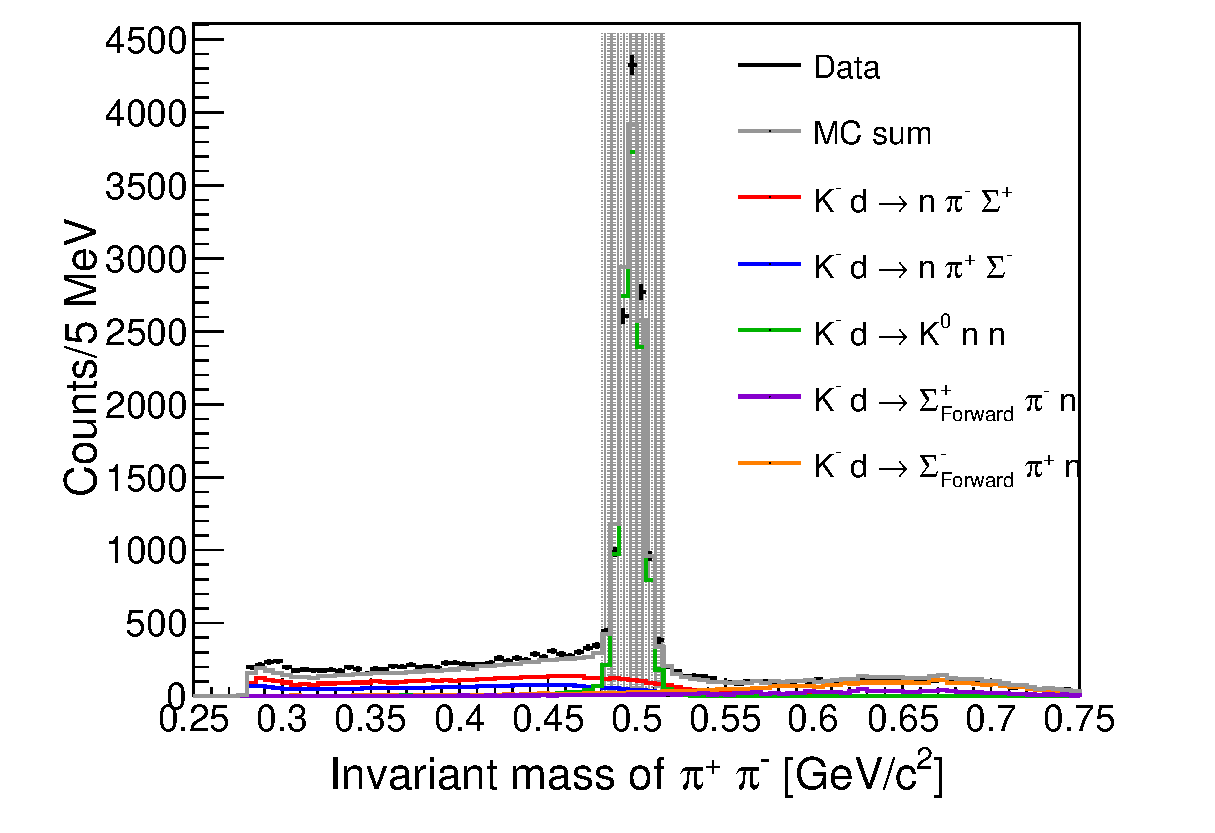
\includegraphics[width=4cm]{../pic/Dron/KN_ana/IM_pipi.eps}
    \end{minipage}
    \begin{minipage}{0.33\hsize}
      \centering
      $n_{forward} \pi^+$ IM\\
      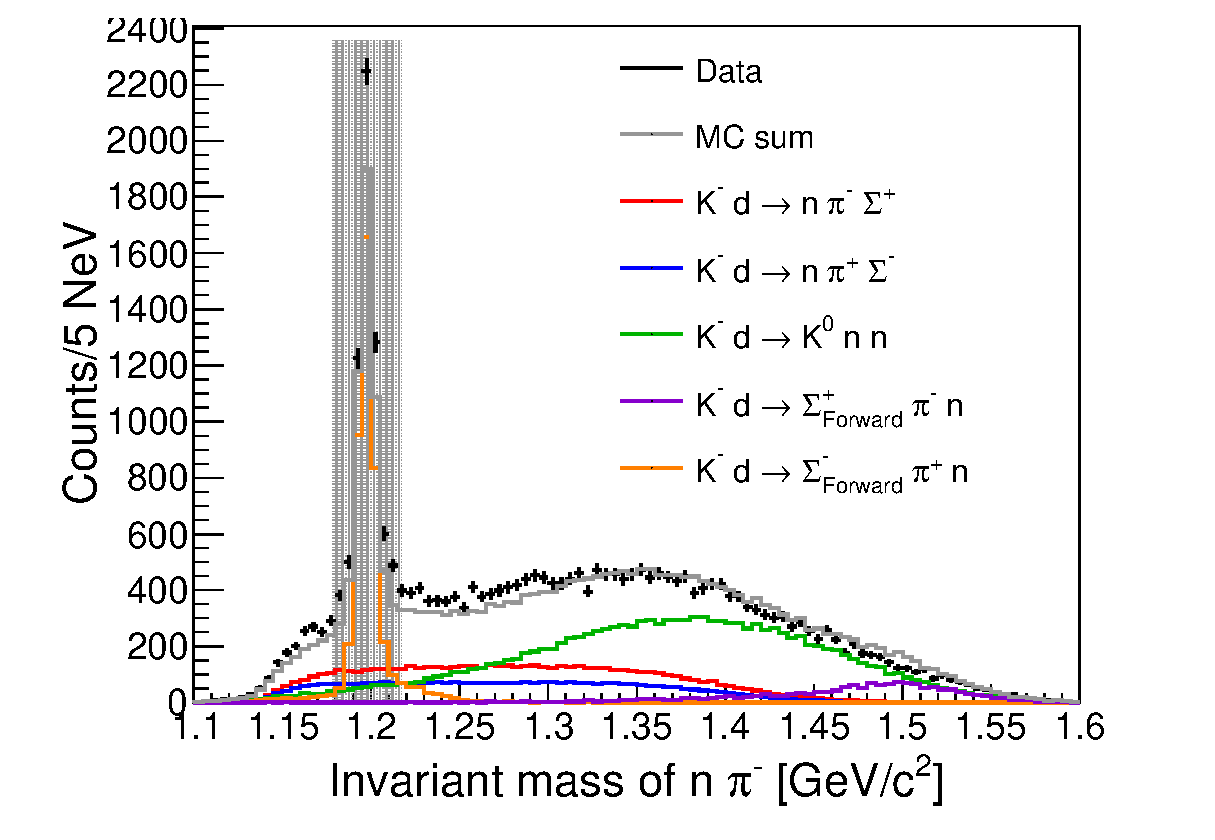
\includegraphics[width=4cm]{../pic/Dron/KN_ana/IM_npim.eps}
    \end{minipage}
    \begin{minipage}{0.33\hsize}
      \centering
      $n_{forward} \pi^-$ IM\\
      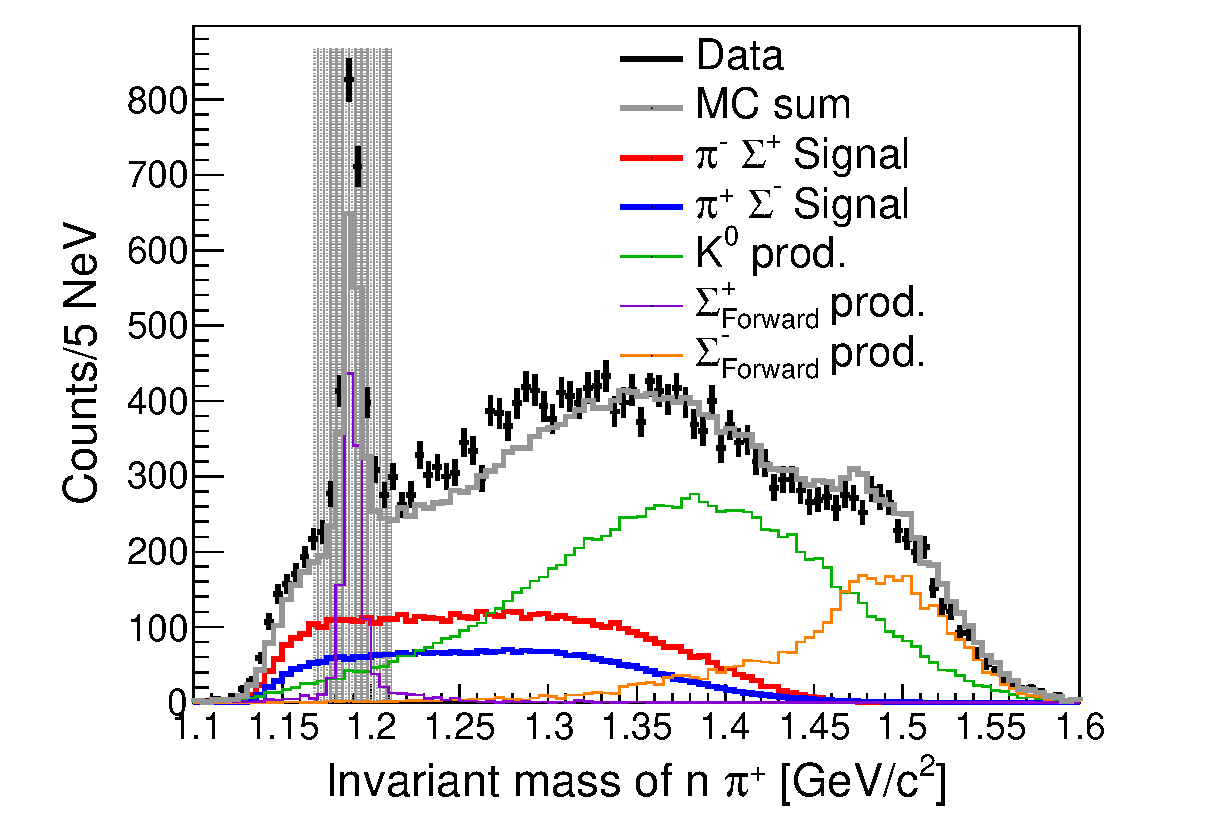
\includegraphics[width=4cm]{../pic/Dron/KN_ana/IM_npip.eps}
    \end{minipage}
  \end{tabular}
  \vspace{4mm}\\
  Each spectra are well reproduced. 
\end{frame}


Next, the fitting procedure for background estimation and  $\pi^{\mp}\Sigma^{\pm}$ separation is explained in detail.
Background fitting is performed using the invariant mass spectra of $\pi^+ \pi^-$, $n_{forward} \pi^+$, and $n_{forward} \pi^-$ 
from all $K^- d \rightarrow n \pi^+ \pi^- n$ final states shown in Figure \ref{fig:npipin_IM_fitGauss}.
The contributions from each process, scaled according to the fitting results, are presented in Figure \ref{fig:fit_IM}.
$K^0$, $\Sigma^+$, and $\Sigma^-$ production are represented by green, purple, and orange lines, respectively,
and produce peaks at the corresponding $\pi^+ \pi^-$, $n_{forward} \pi^+$, and $n_{forward} \pi^-$ invariant masses.
The backward $\pi^- \Sigma^+$ and $\pi^+ \Sigma^-$ scattering signals are shown in red and blue lines, respectively,
and are uniformly distributed without peaks at these invariant masses.

The fact that these invariant mass distributions are reproduced using templates generated by the Monte Carlo simulation indicates
that the $K^- d \rightarrow n \pi^+ \pi^- n$ final state can be decomposed into the signal and $K^0$ and $\Sigma^{\pm}_{forward}$ production components.
In template fitting, it is known that $-2\ln(\Lambda)$ asymptotically approaches $\chi^2$ in the limit of an infinite number of samples,
where $\Lambda$ denotes the likelihood.
In this fitting, $-2\ln(\Lambda)/NDF \sim \chi^2/NDF = \IMfitChiSquare/\IMfitNDF = \IMfitChiNDF$.

\begin{figure}[htbp]
  \centering
  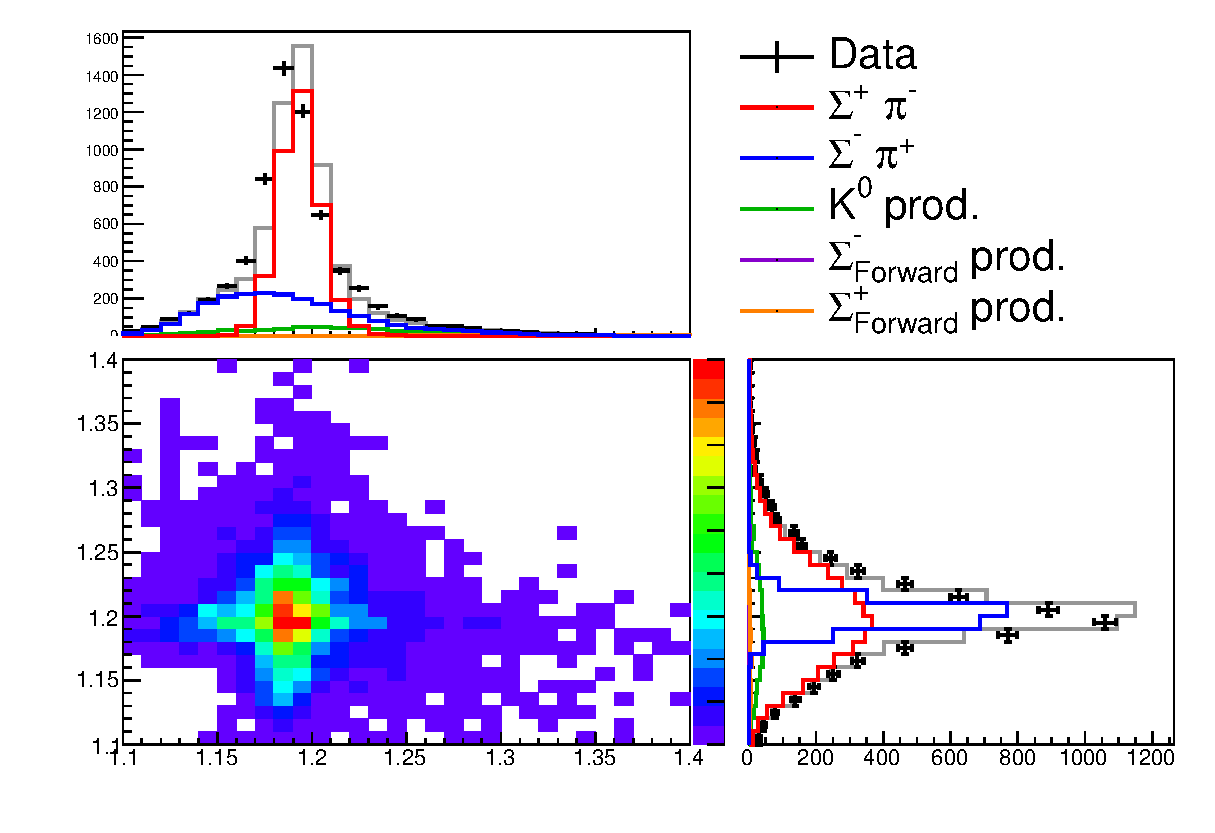
\includegraphics[width=12cm]{../pic/Run78/KN_ana_NC170_2sigma/KNpim_KNpip_MM.eps}
  \caption{
    This figure shows template fitting of the $d(K^-, n \pi)$ spectra to separate the $\pi^-\Sigma^+$ and $\pi^+ \Sigma^-$ modes.
    The lower left figure shows two-dimensional plots of $d(K^-, n \pi^-)$ and $d(K^-, n \pi^+)$ on the horizontal and vertical axes, respectively.
    The top and right panels show the projections onto each axis.
    The caption is the same as that of Figure.\ref{fig:fit_IM}.
  }
  \label{fig:fit_KNpi_MM_all}
\end{figure}

\begin{figure}
  \begin{tabular}{ccccc}
    \begin{minipage}{0.2\hsize}
      \includegraphics[width=2.2cm]{../pic/Run78/KN_ana_NC170_2sigma/KNpi_MM_0.eps}
    \end{minipage}
    \begin{minipage}{0.2\hsize}
      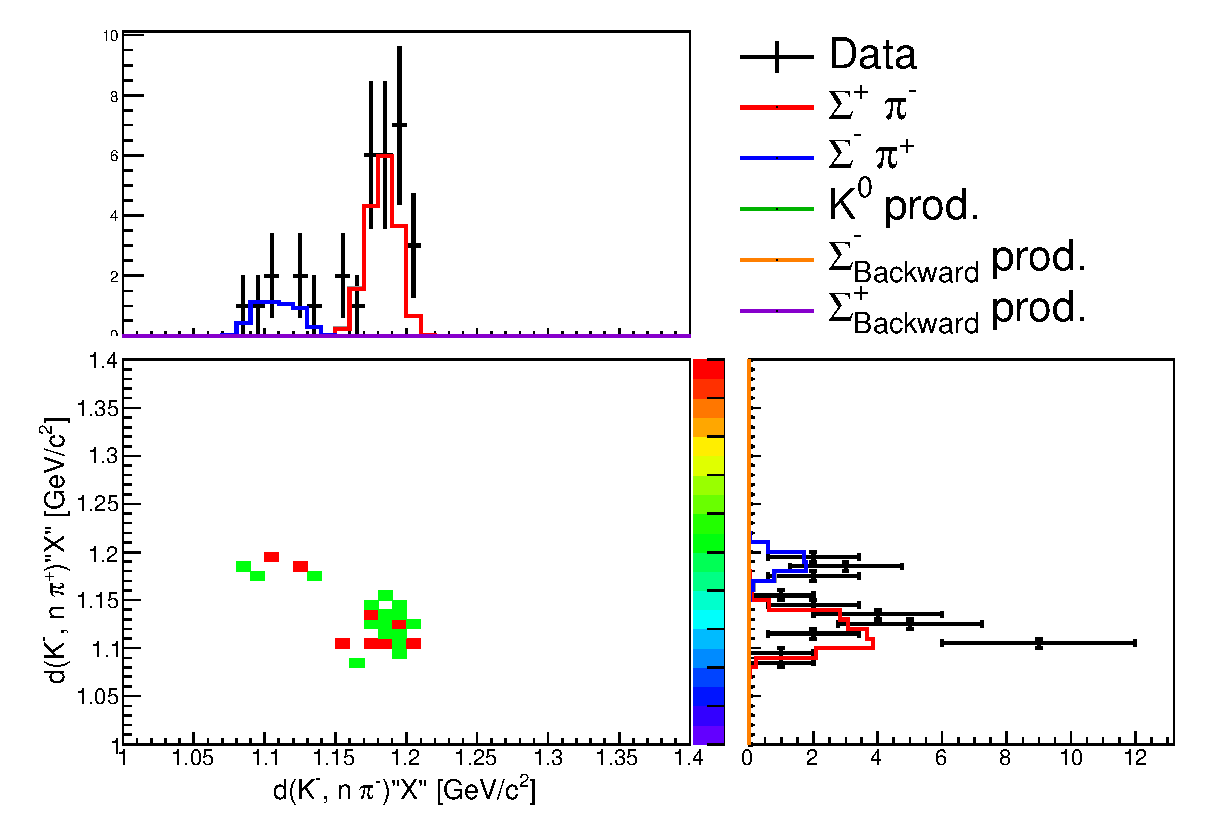
\includegraphics[width=2.2cm]{../pic/Run78/KN_ana_NC170_2sigma/KNpi_MM_1.eps}
    \end{minipage}
    \begin{minipage}{0.2\hsize}
      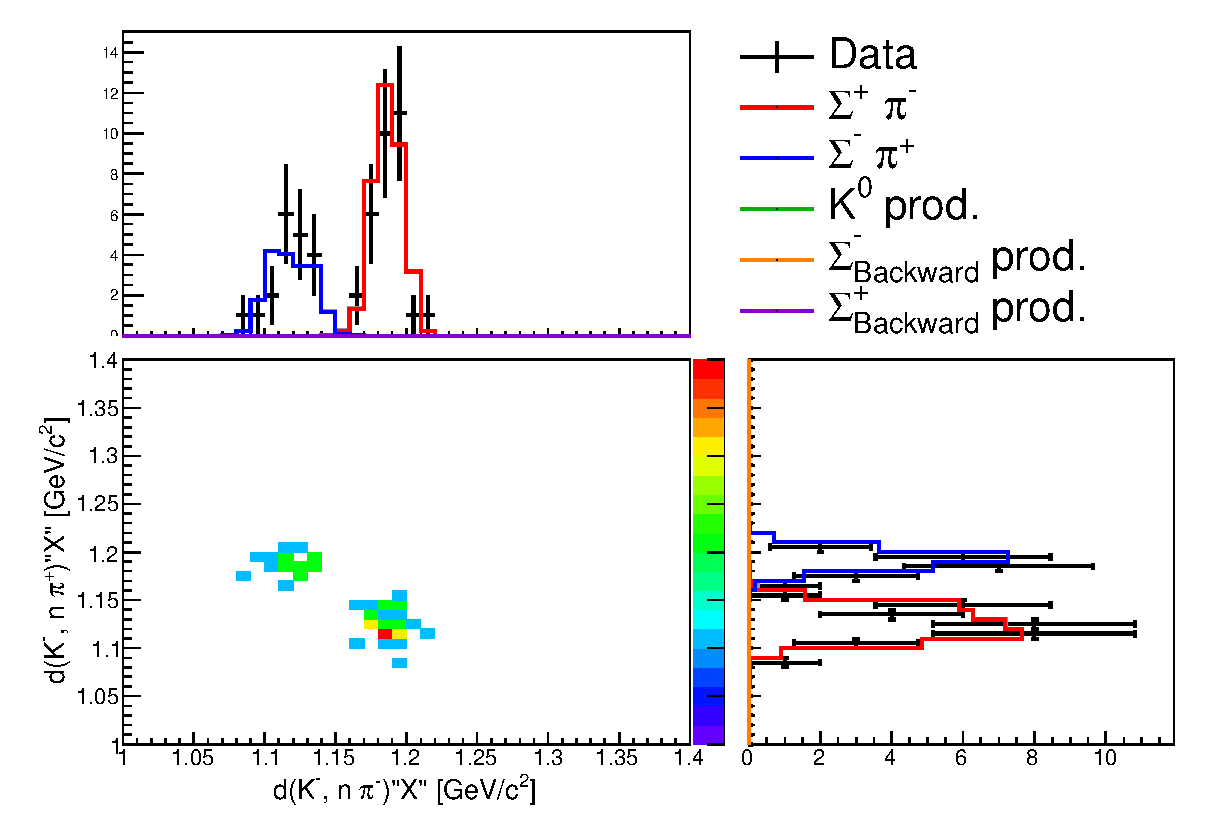
\includegraphics[width=2.2cm]{../pic/Run78/KN_ana_NC170_2sigma/KNpi_MM_2.eps}
    \end{minipage}
    \begin{minipage}{0.2\hsize}
      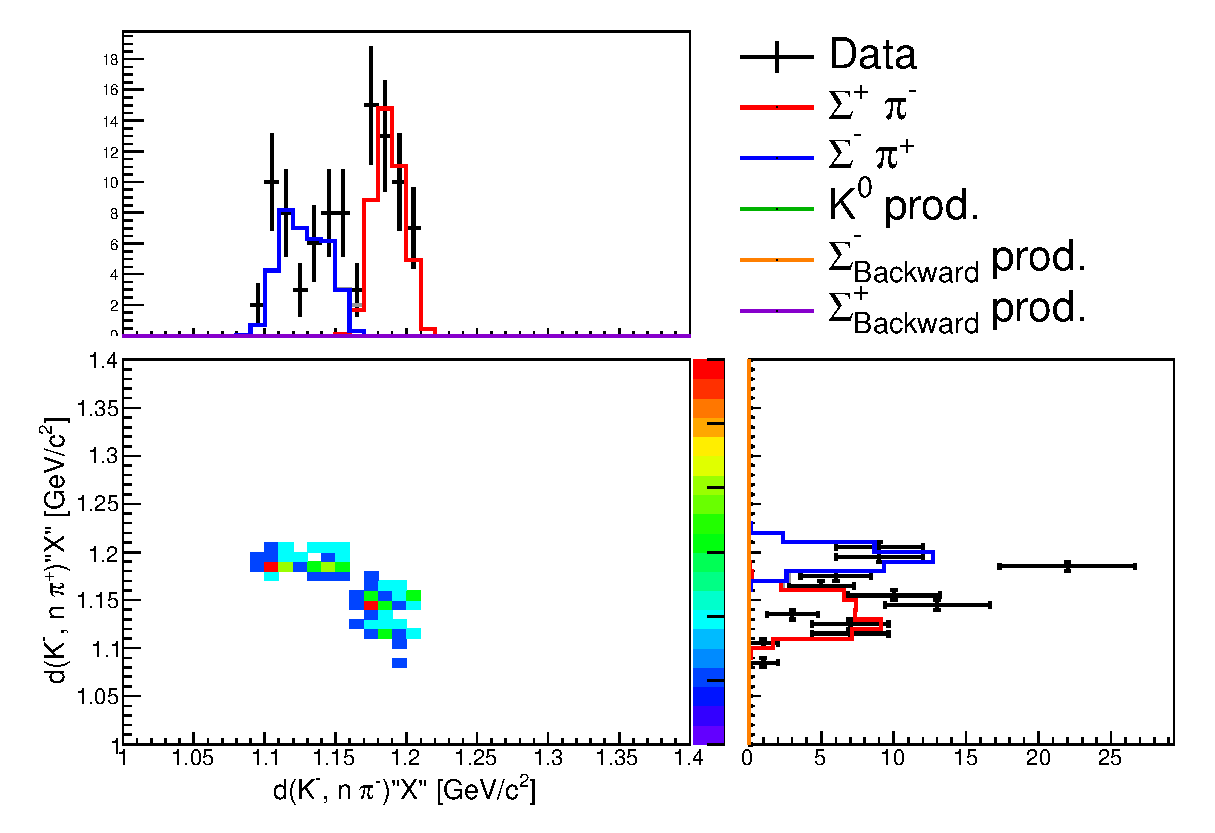
\includegraphics[width=2.2cm]{../pic/Run78/KN_ana_NC170_2sigma/KNpi_MM_3.eps}
    \end{minipage}
    \begin{minipage}{0.2\hsize}
      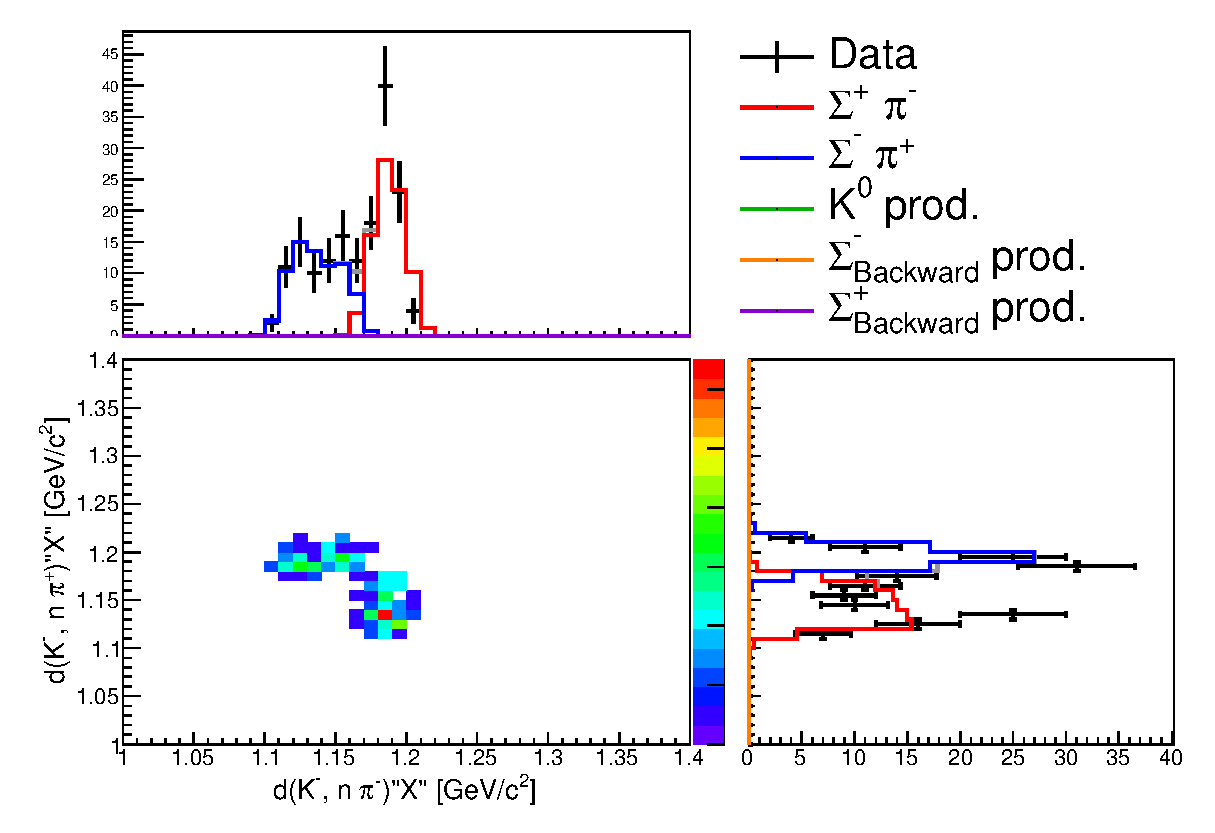
\includegraphics[width=2.2cm]{../pic/Run78/KN_ana_NC170_2sigma/KNpi_MM_4.eps}
    \end{minipage}
  \end{tabular}
  \begin{tabular}{ccccc}
    \begin{minipage}{0.2\hsize}
      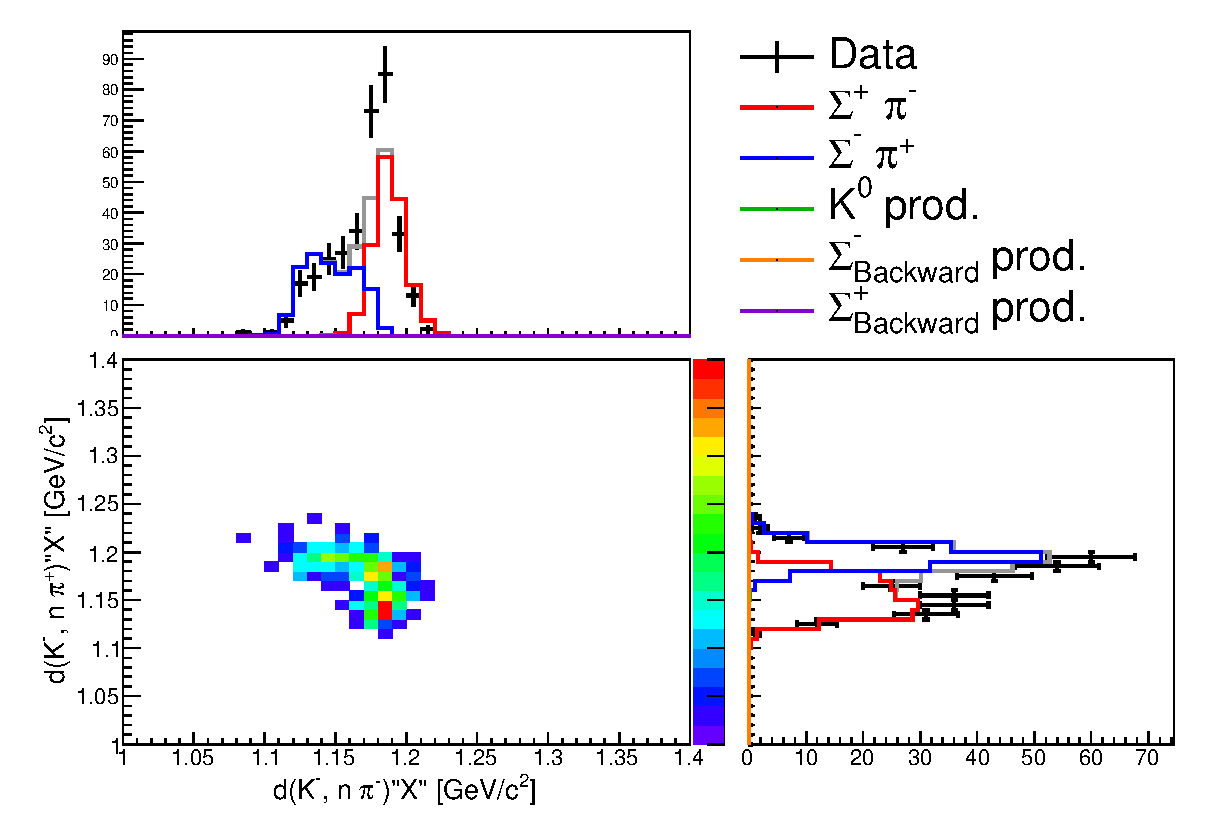
\includegraphics[width=2.2cm]{../pic/Run78/KN_ana_NC170_2sigma/KNpi_MM_5.eps}
    \end{minipage}
    \begin{minipage}{0.2\hsize}
      \includegraphics[width=2.2cm]{../pic/Run78/KN_ana_NC170_2sigma/KNpi_MM_6.eps}
    \end{minipage}
    \begin{minipage}{0.2\hsize}
      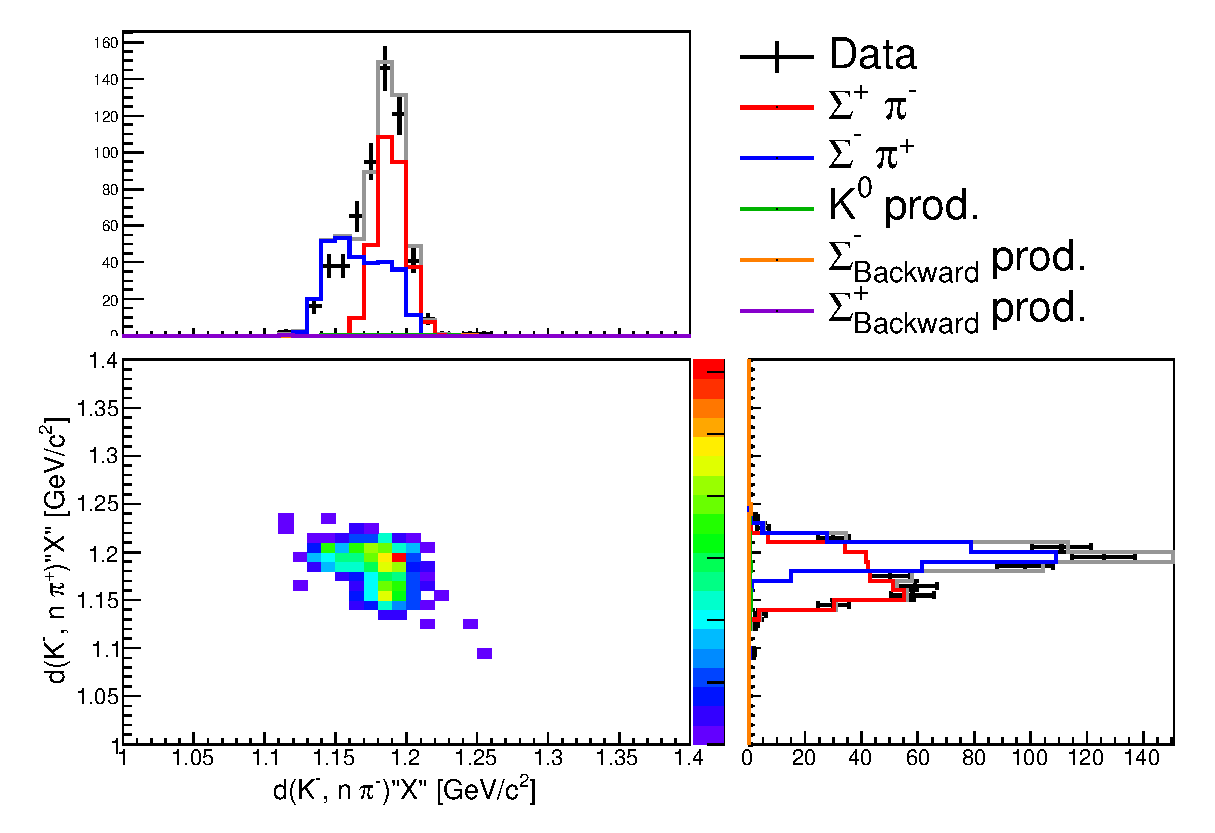
\includegraphics[width=2.2cm]{../pic/Run78/KN_ana_NC170_2sigma/KNpi_MM_7.eps}
    \end{minipage}
    \begin{minipage}{0.2\hsize}
      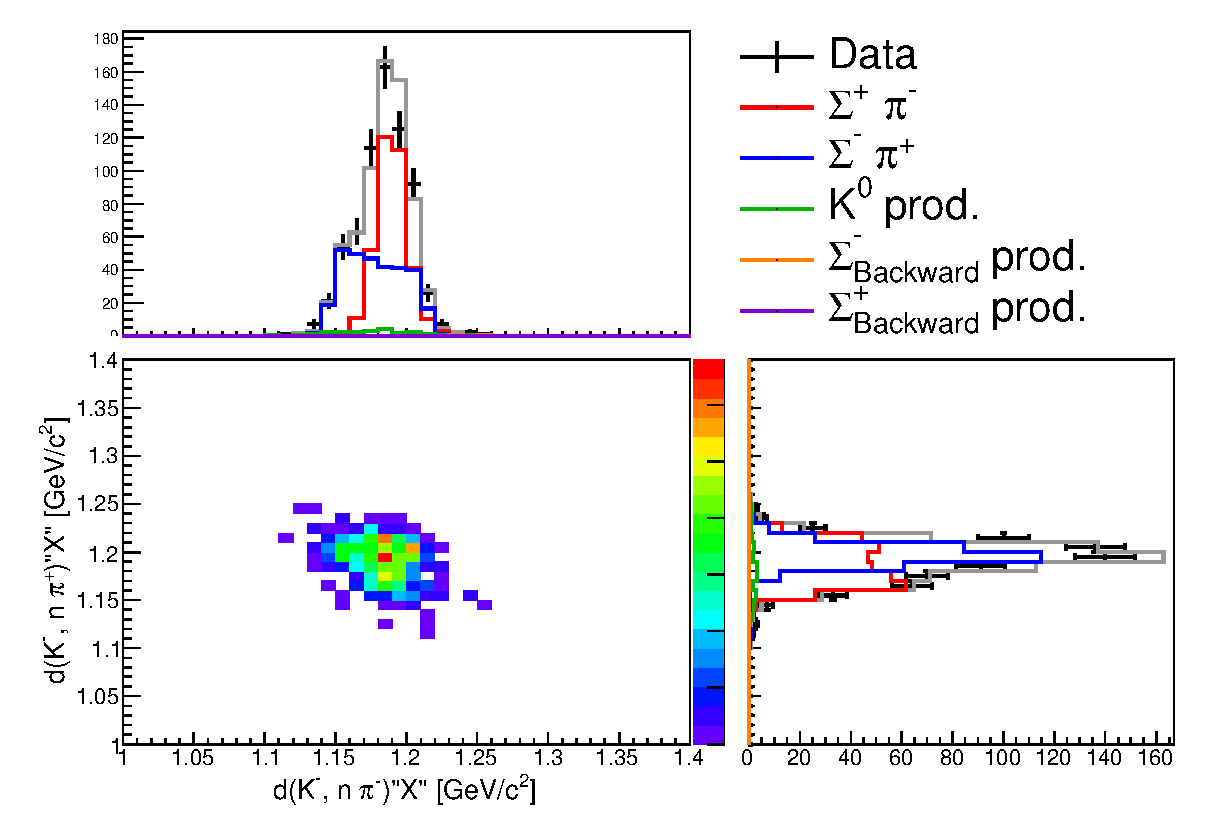
\includegraphics[width=2.2cm]{../pic/Run78/KN_ana_NC170_2sigma/KNpi_MM_8.eps}
    \end{minipage}
    \begin{minipage}{0.2\hsize}
      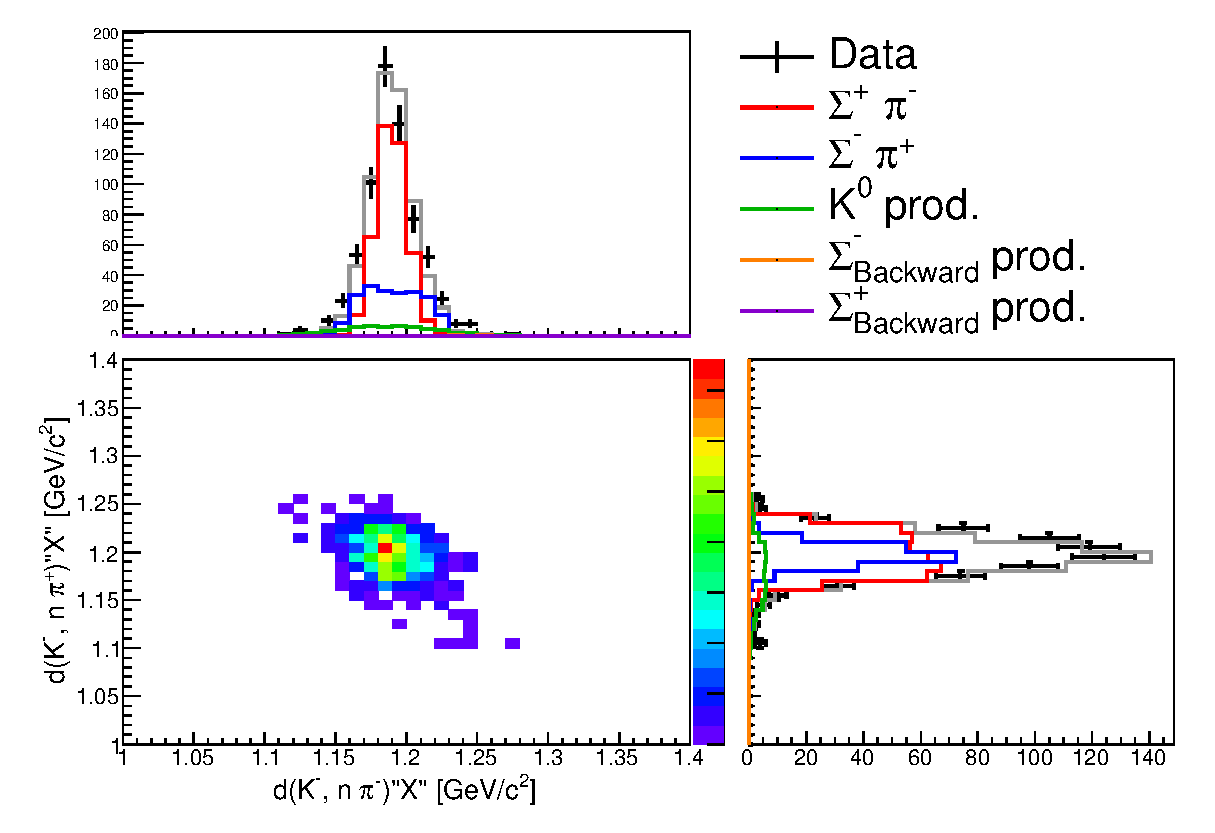
\includegraphics[width=2.2cm]{../pic/Run78/KN_ana_NC170_2sigma/KNpi_MM_9.eps}
    \end{minipage}
  \end{tabular}
  \begin{tabular}{ccccc}
    \begin{minipage}{0.2\hsize}
      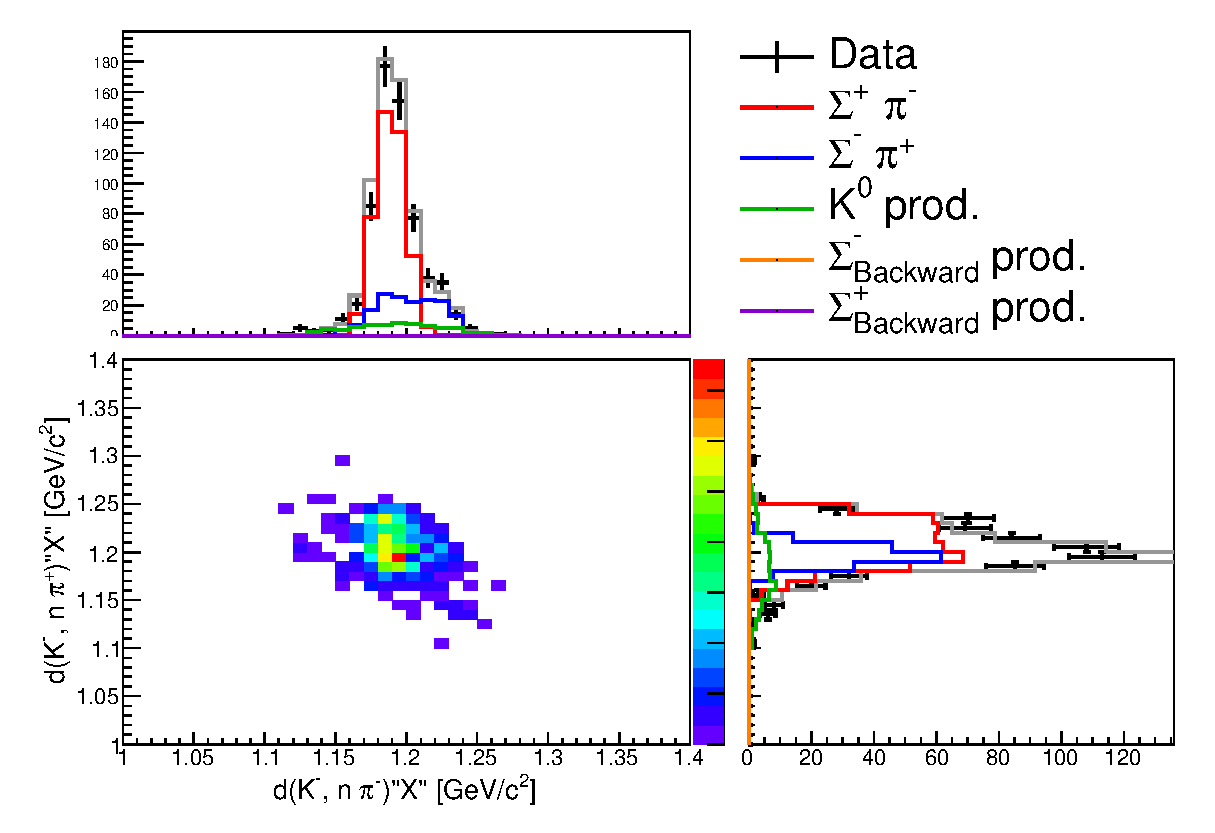
\includegraphics[width=2.2cm]{../pic/Run78/KN_ana_NC170_2sigma/KNpi_MM_10.eps}
    \end{minipage}
    \begin{minipage}{0.2\hsize}
      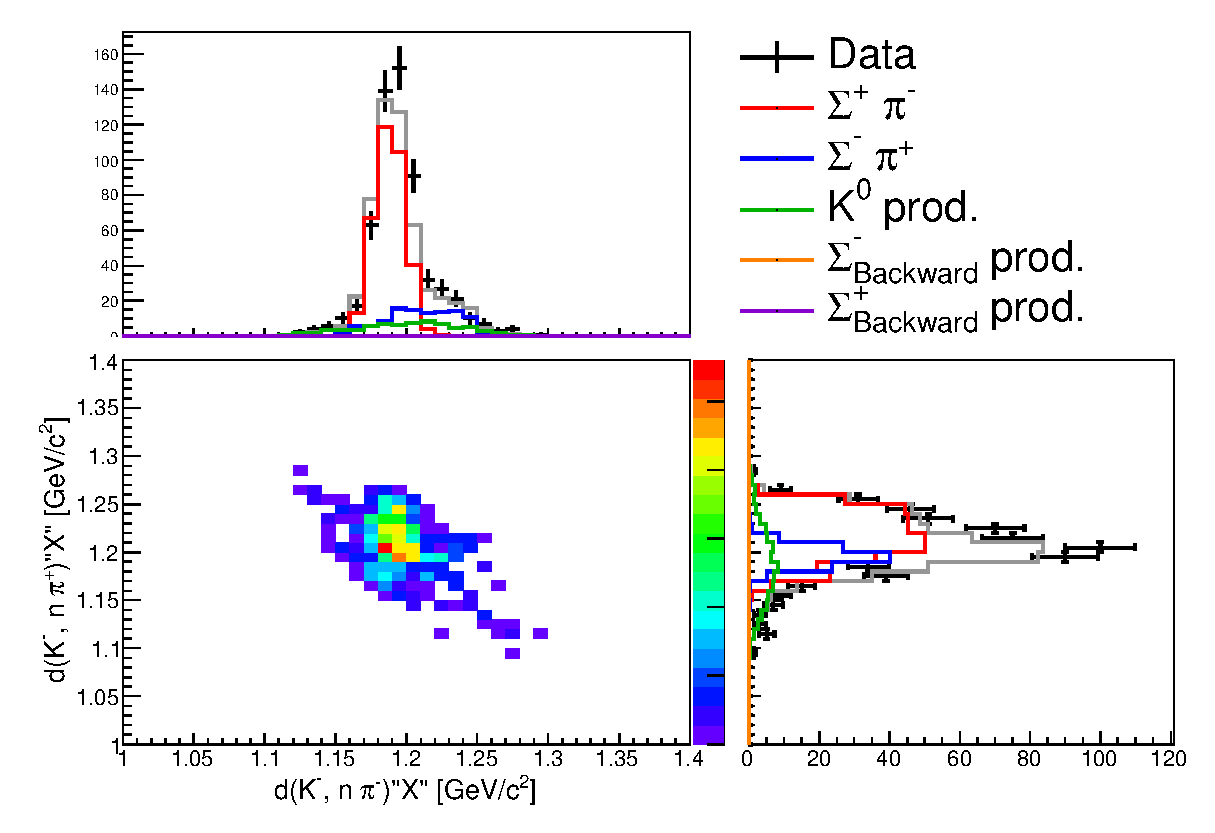
\includegraphics[width=2.2cm]{../pic/Run78/KN_ana_NC170_2sigma/KNpi_MM_11.eps}
    \end{minipage}
    \begin{minipage}{0.2\hsize}
      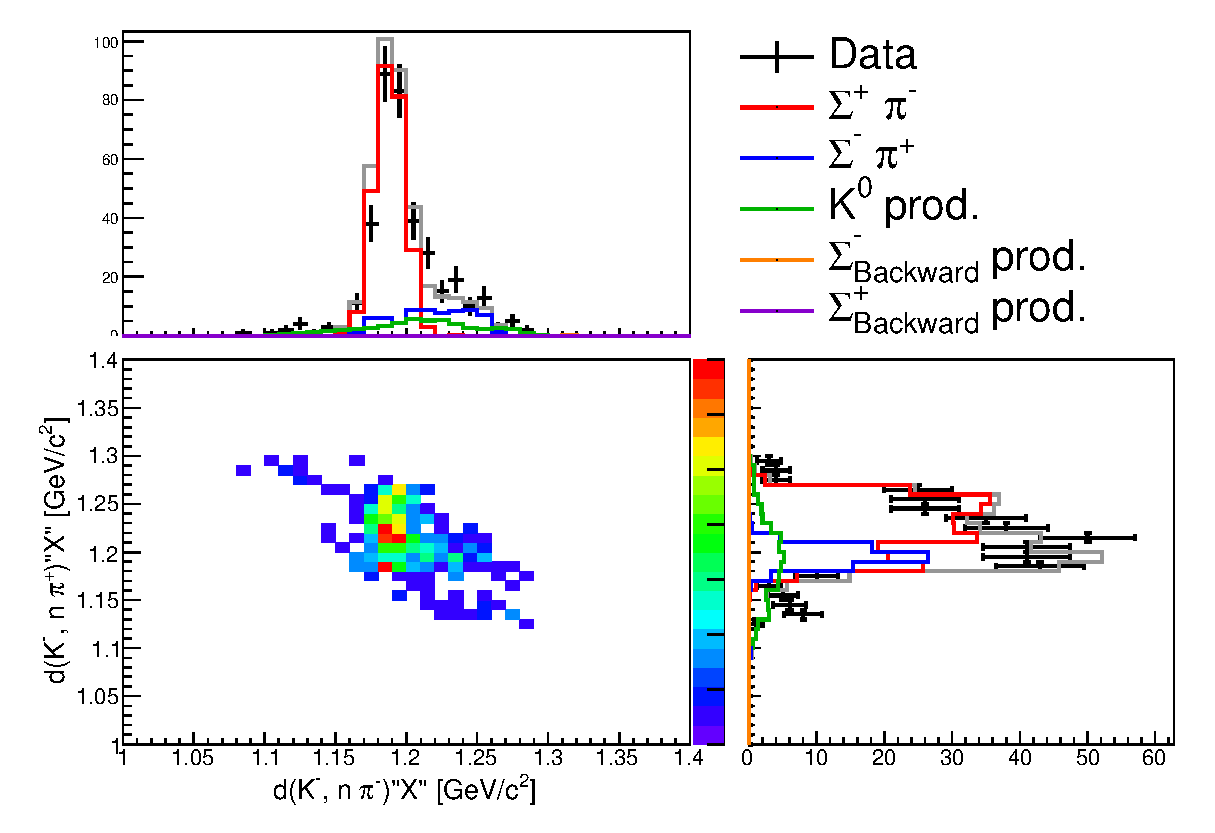
\includegraphics[width=2.2cm]{../pic/Run78/KN_ana_NC170_2sigma/KNpi_MM_12.eps}
    \end{minipage}
    \begin{minipage}{0.2\hsize}
      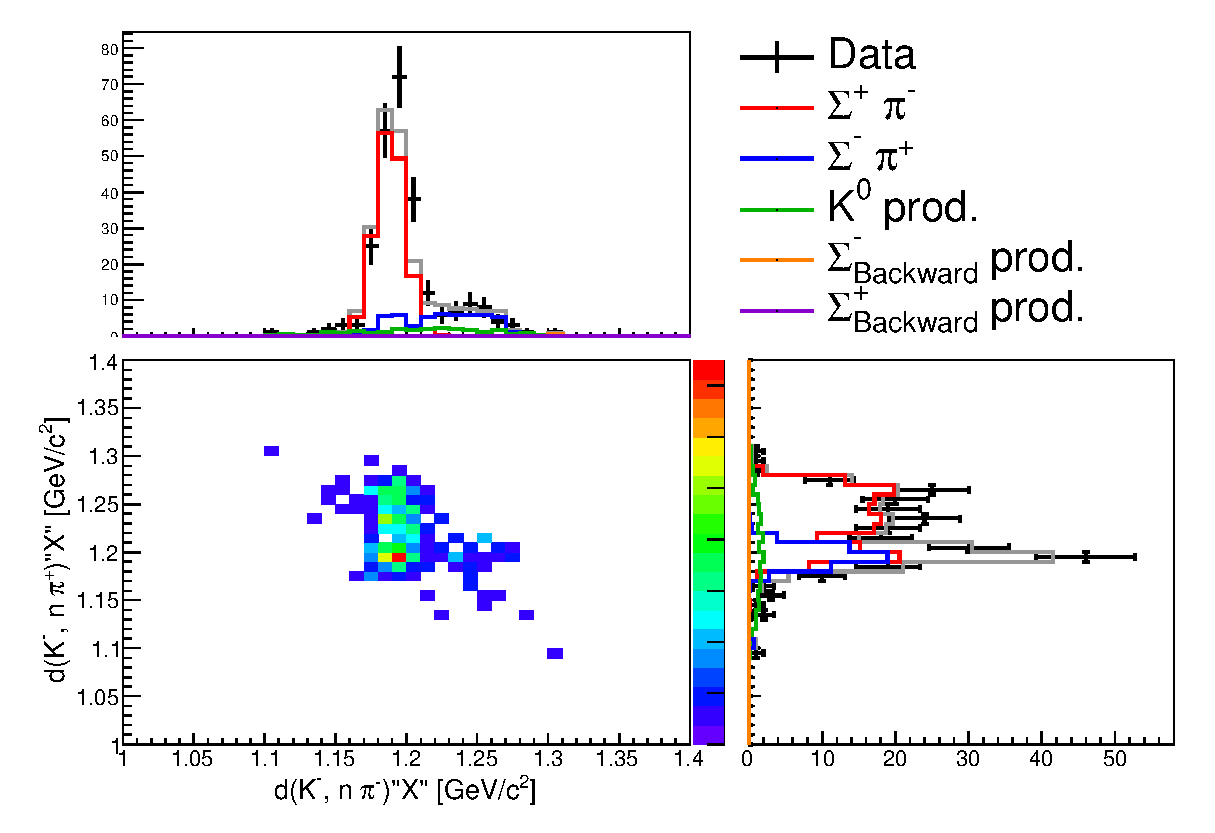
\includegraphics[width=2.2cm]{../pic/Run78/KN_ana_NC170_2sigma/KNpi_MM_13.eps}
    \end{minipage}
    \begin{minipage}{0.2\hsize}
      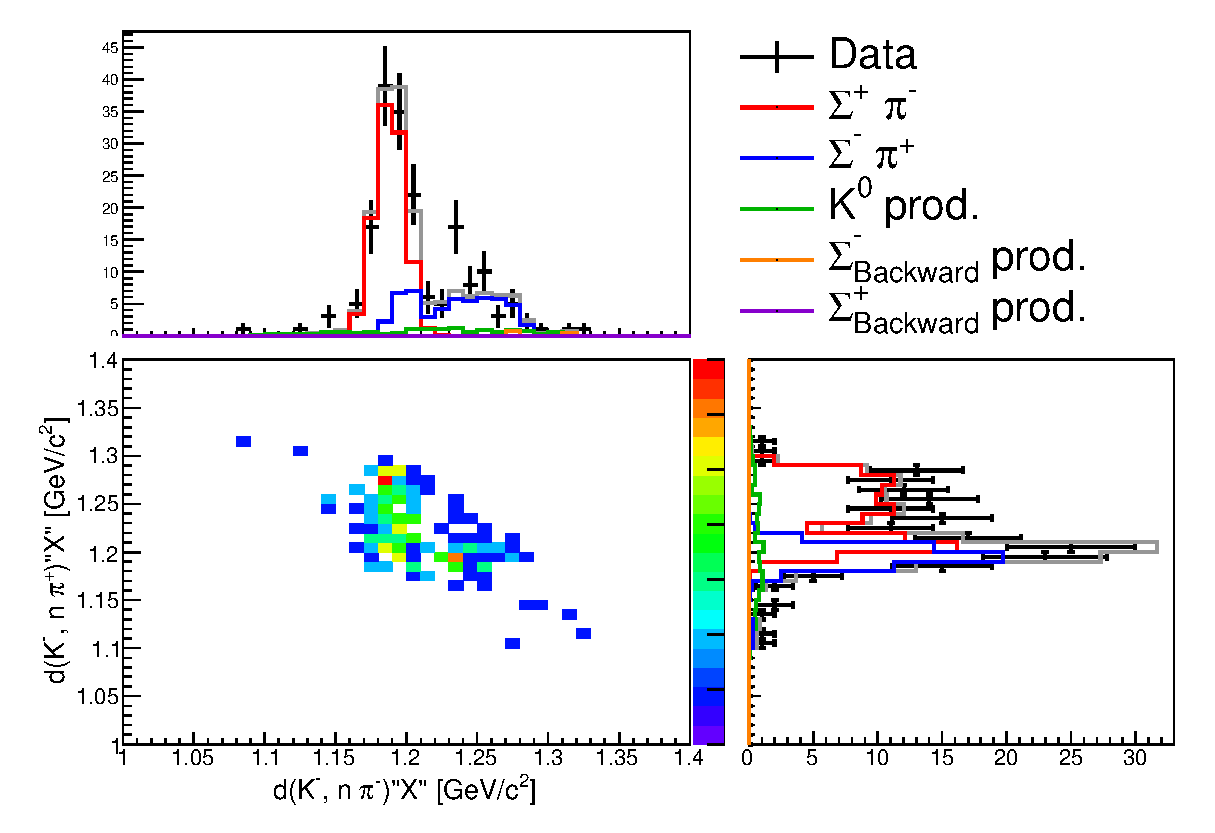
\includegraphics[width=2.2cm]{../pic/Run78/KN_ana_NC170_2sigma/KNpi_MM_14.eps}
    \end{minipage}
  \end{tabular}
  \begin{tabular}{ccccc}
    \begin{minipage}{0.2\hsize}
      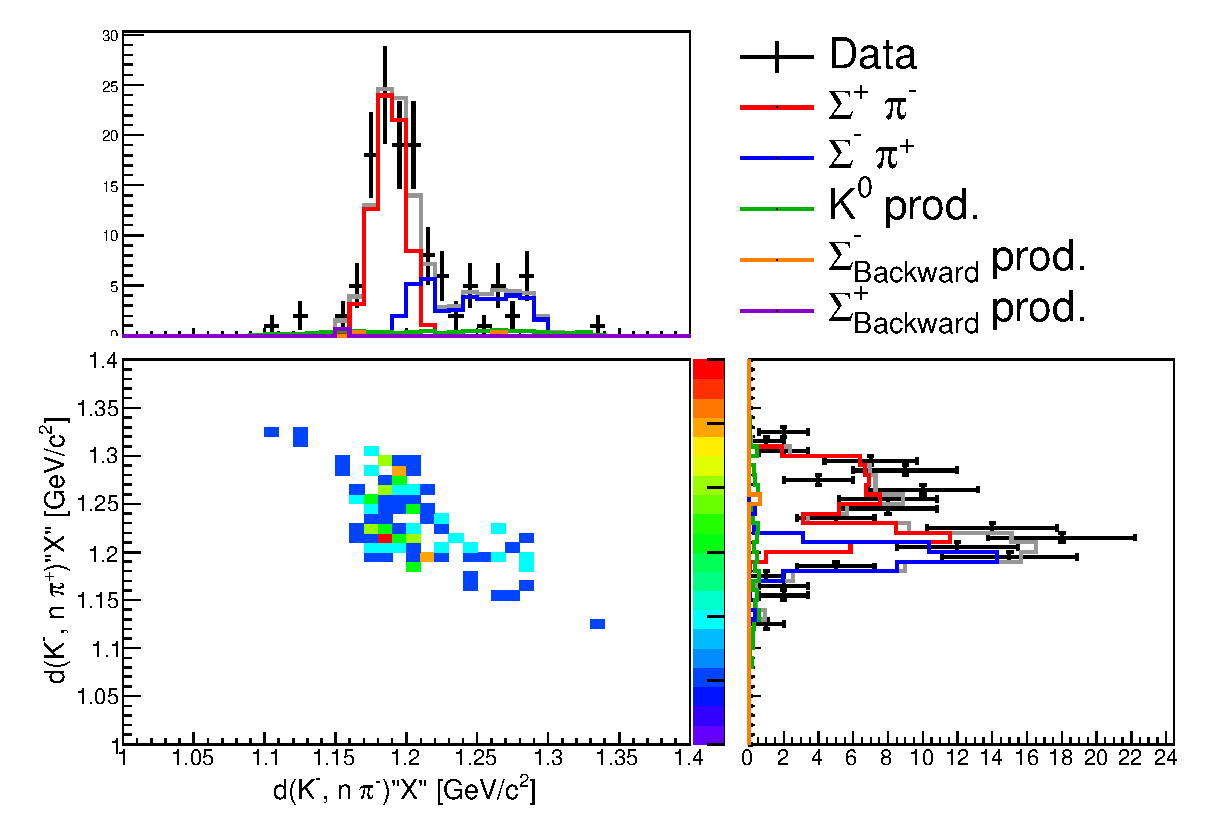
\includegraphics[width=2.2cm]{../pic/Run78/KN_ana_NC170_2sigma/KNpi_MM_15.eps}
    \end{minipage}
    \begin{minipage}{0.2\hsize}
      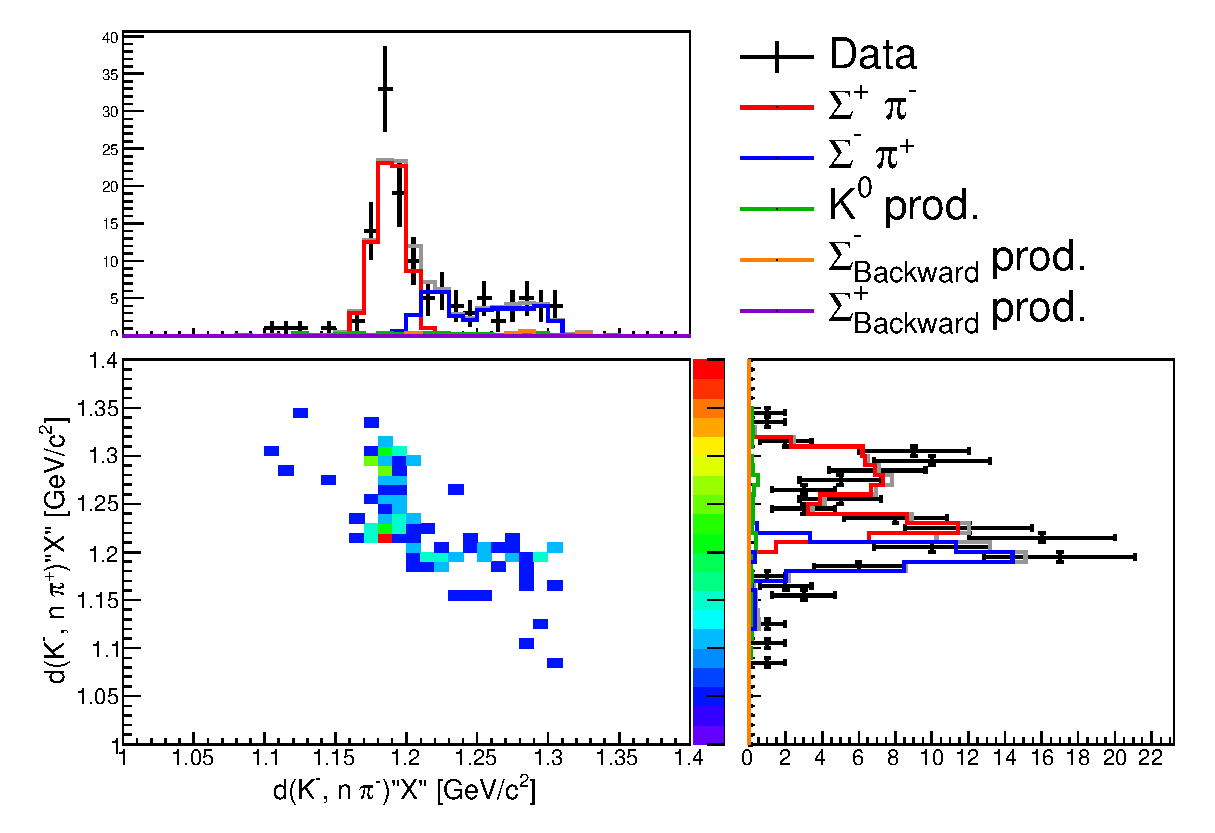
\includegraphics[width=2.2cm]{../pic/Run78/KN_ana_NC170_2sigma/KNpi_MM_16.eps}
    \end{minipage}
    \begin{minipage}{0.2\hsize}
      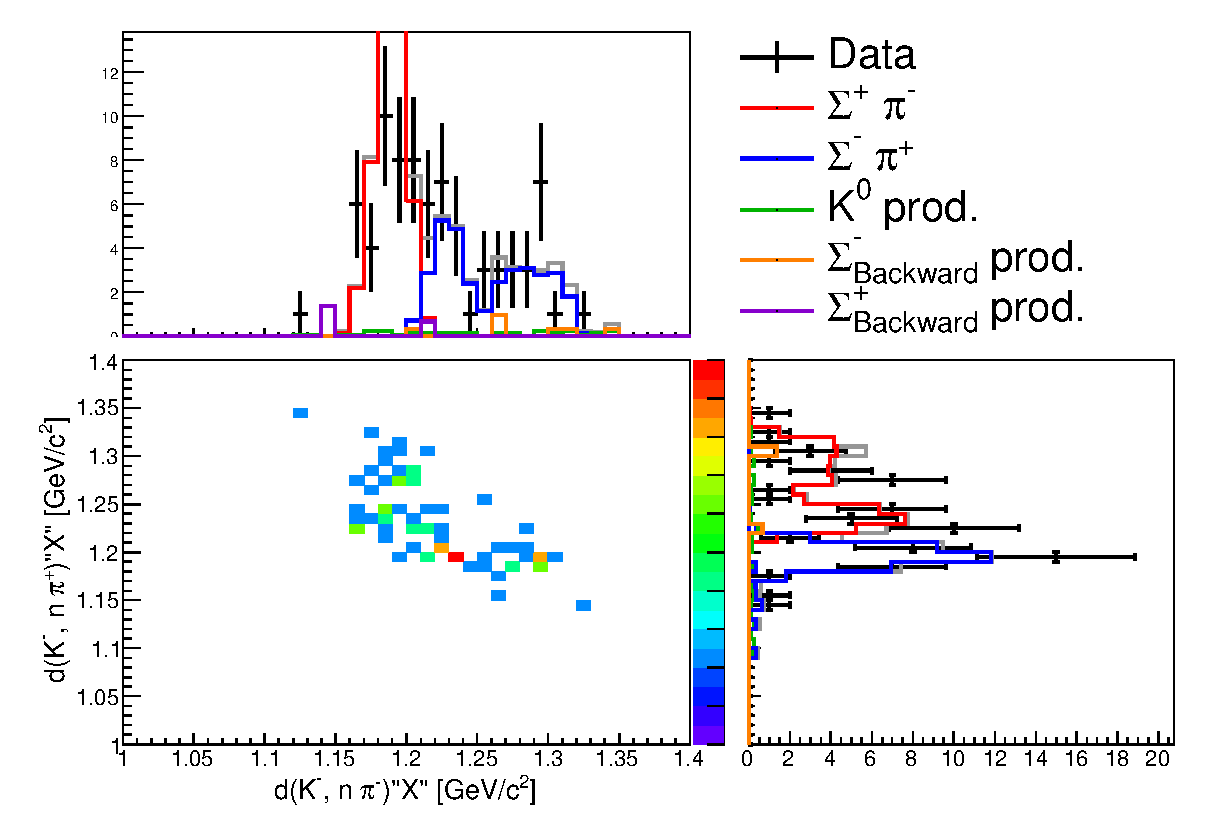
\includegraphics[width=2.2cm]{../pic/Run78/KN_ana_NC170_2sigma/KNpi_MM_17.eps}
    \end{minipage}
    \begin{minipage}{0.2\hsize}
      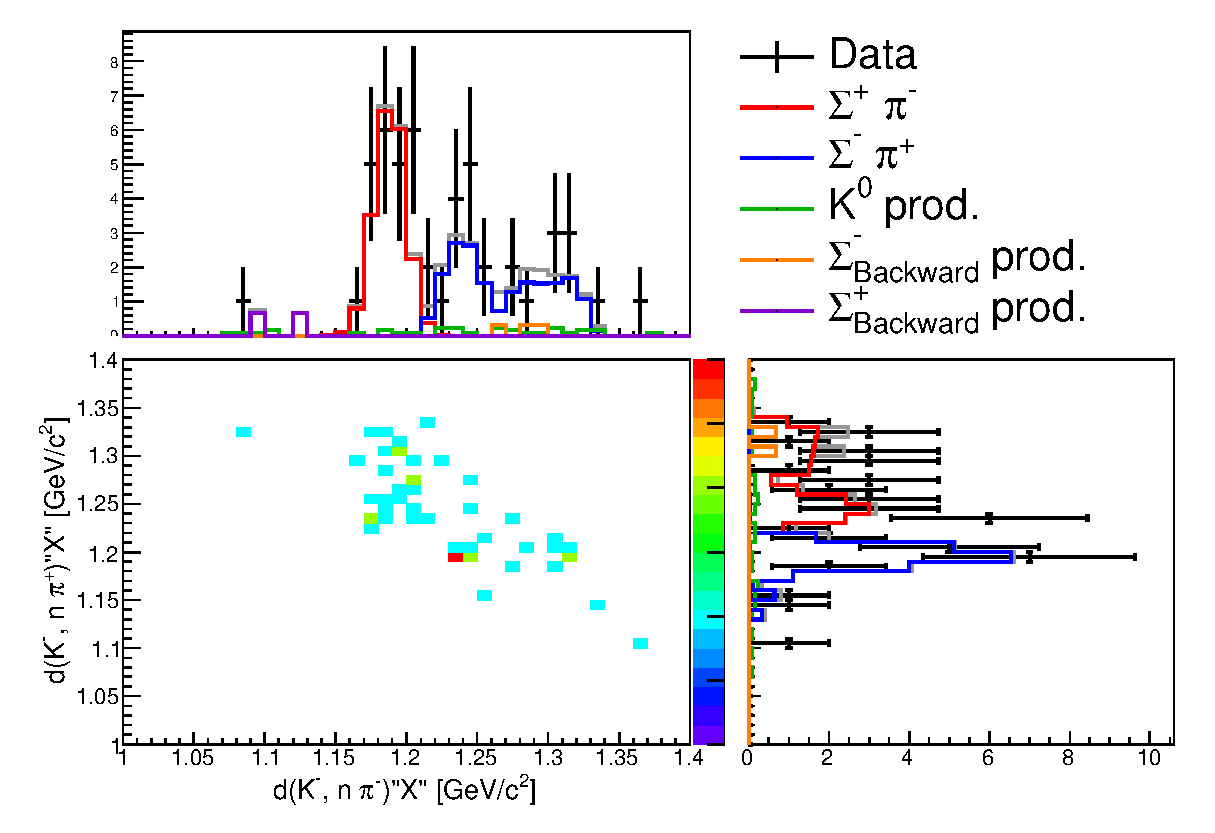
\includegraphics[width=2.2cm]{../pic/Run78/KN_ana_NC170_2sigma/KNpi_MM_18.eps}
    \end{minipage}
    \begin{minipage}{0.2\hsize}
      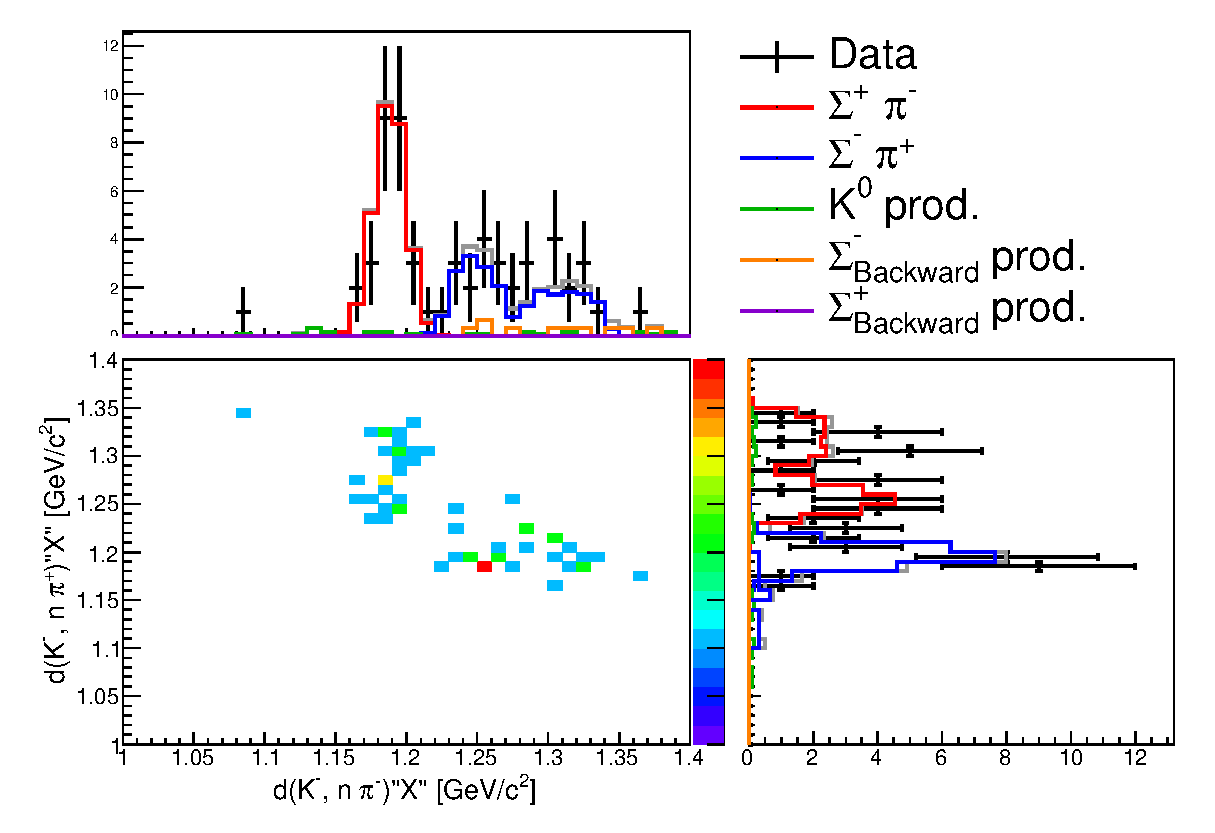
\includegraphics[width=2.2cm]{../pic/Run78/KN_ana_NC170_2sigma/KNpi_MM_19.eps}
    \end{minipage}
  \end{tabular}
  \begin{tabular}{ccccc}
    \begin{minipage}{0.2\hsize}
      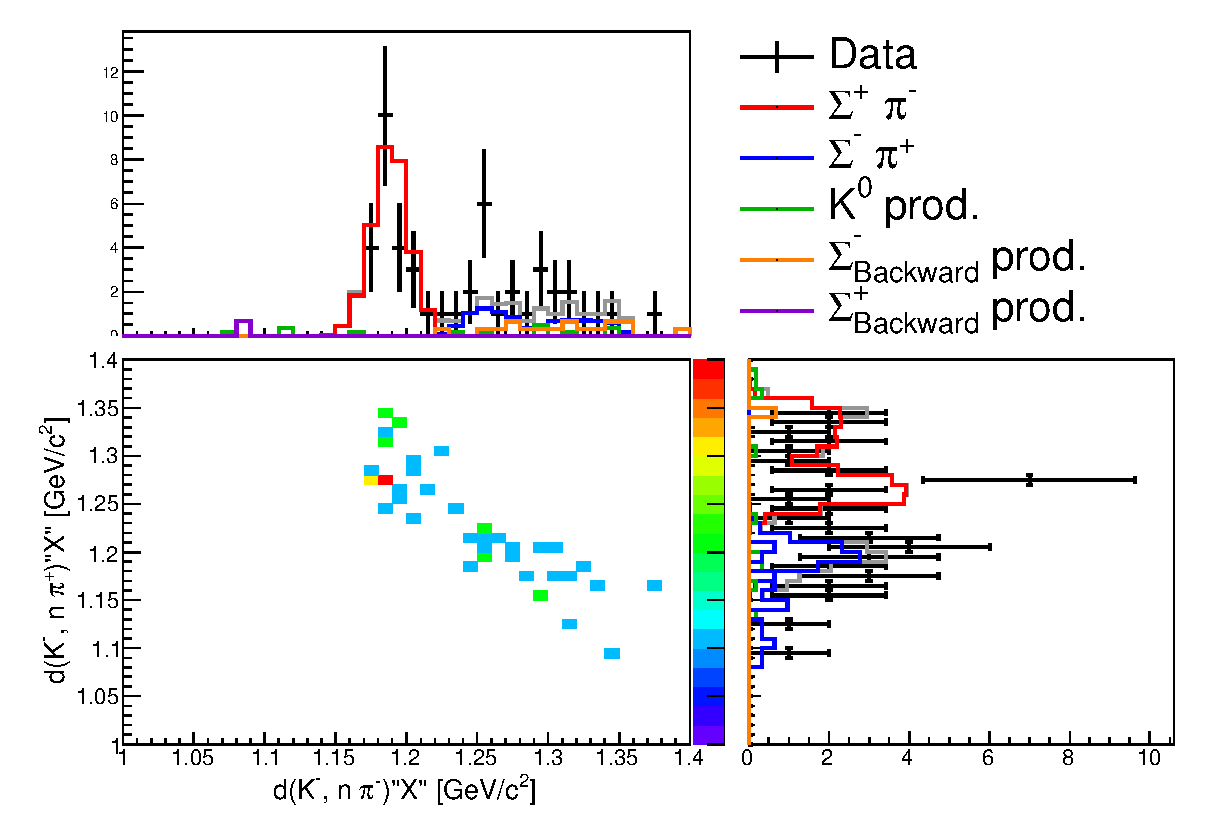
\includegraphics[width=2.2cm]{../pic/Run78/KN_ana_NC170_2sigma/KNpi_MM_20.eps}
    \end{minipage}
    \begin{minipage}{0.2\hsize}
      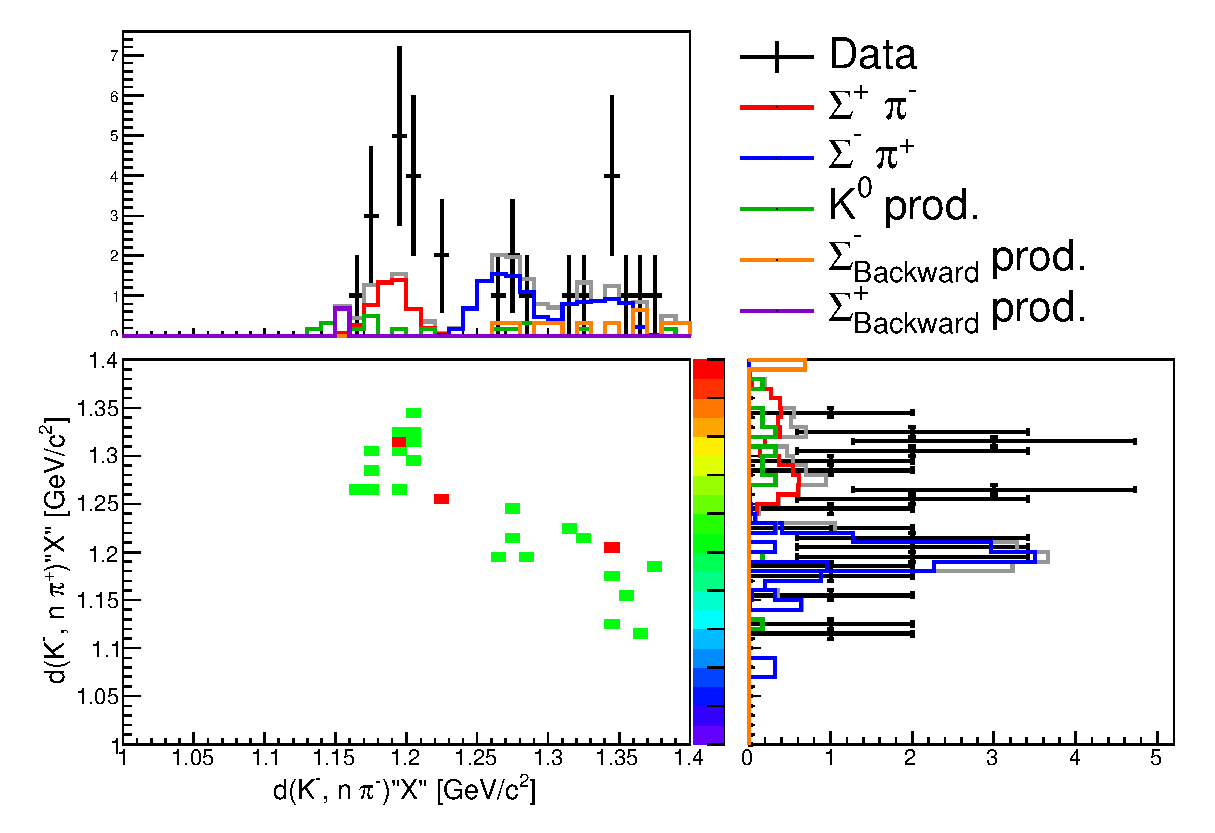
\includegraphics[width=2.2cm]{../pic/Run78/KN_ana_NC170_2sigma/KNpi_MM_21.eps}
    \end{minipage}
    \begin{minipage}{0.2\hsize}
      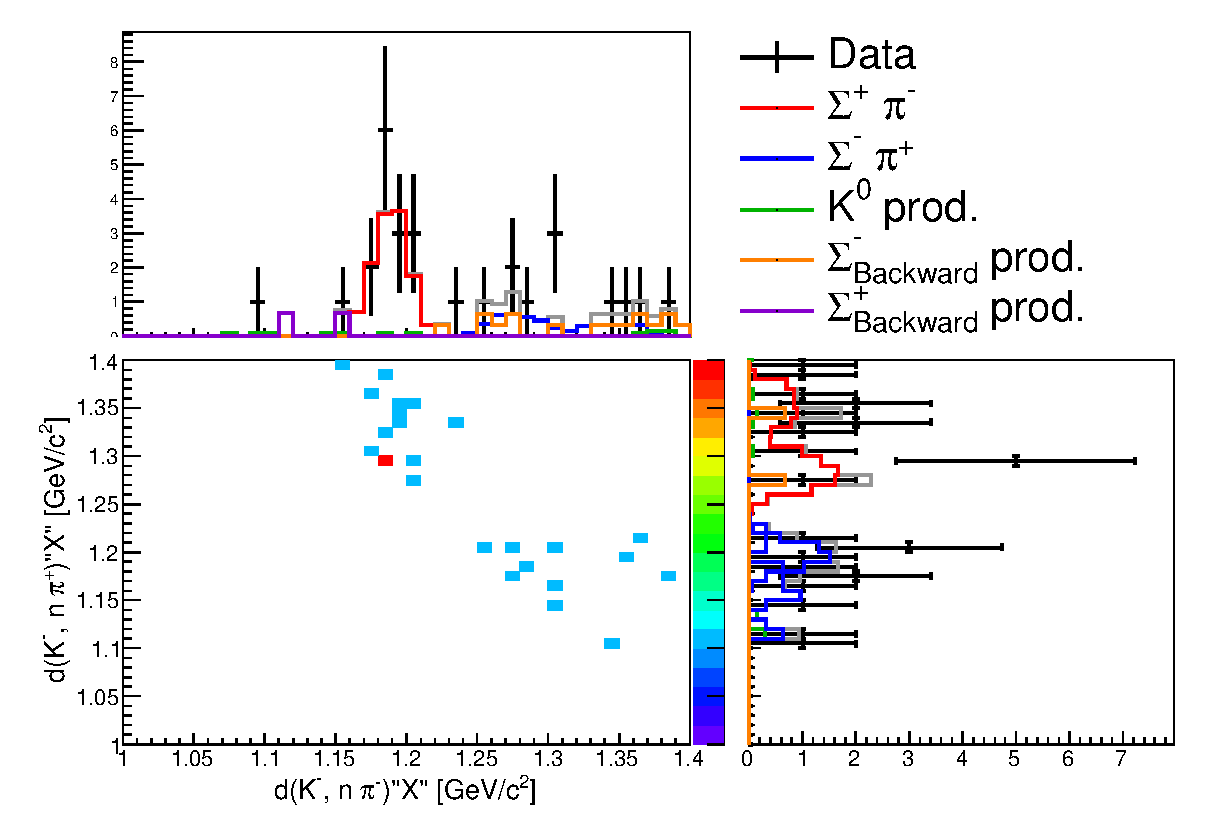
\includegraphics[width=2.2cm]{../pic/Run78/KN_ana_NC170_2sigma/KNpi_MM_22.eps}
    \end{minipage}
    \begin{minipage}{0.2\hsize}
      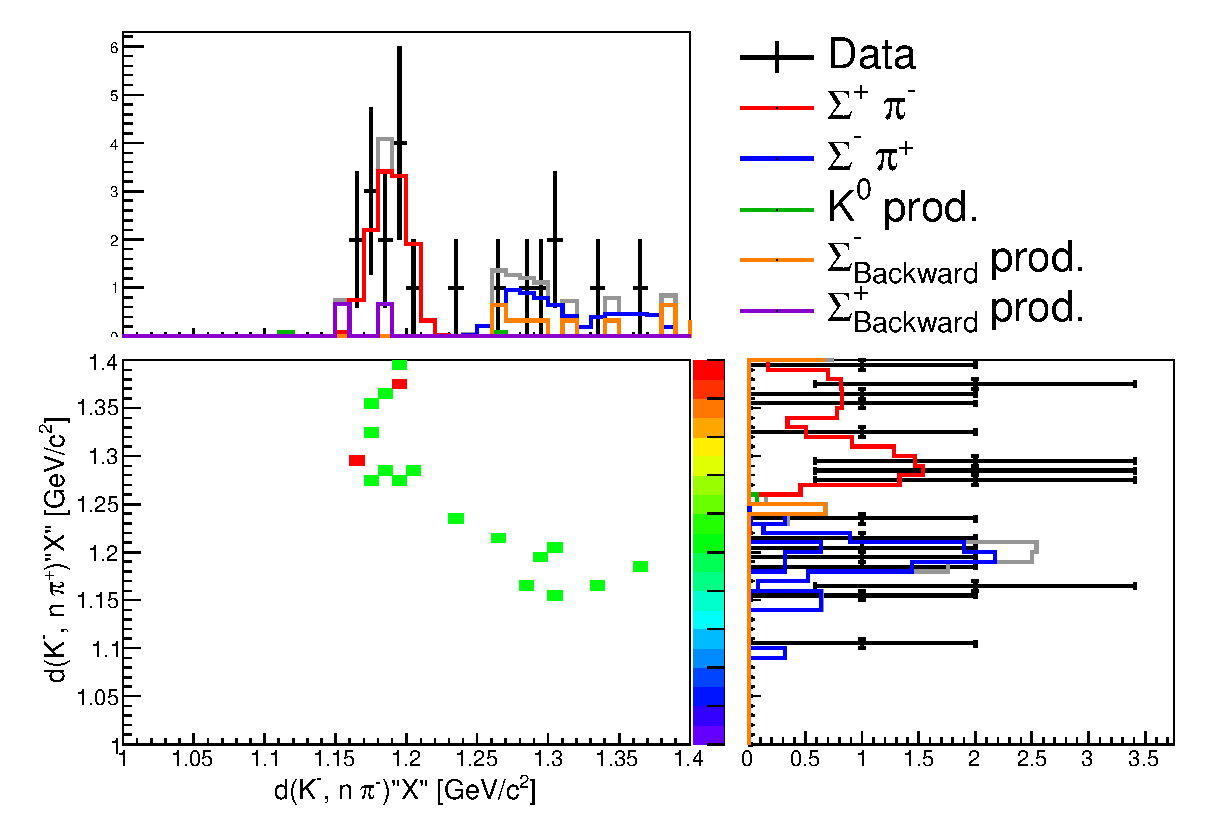
\includegraphics[width=2.2cm]{../pic/Run78/KN_ana_NC170_2sigma/KNpi_MM_23.eps}
    \end{minipage}
    \begin{minipage}{0.2\hsize}
      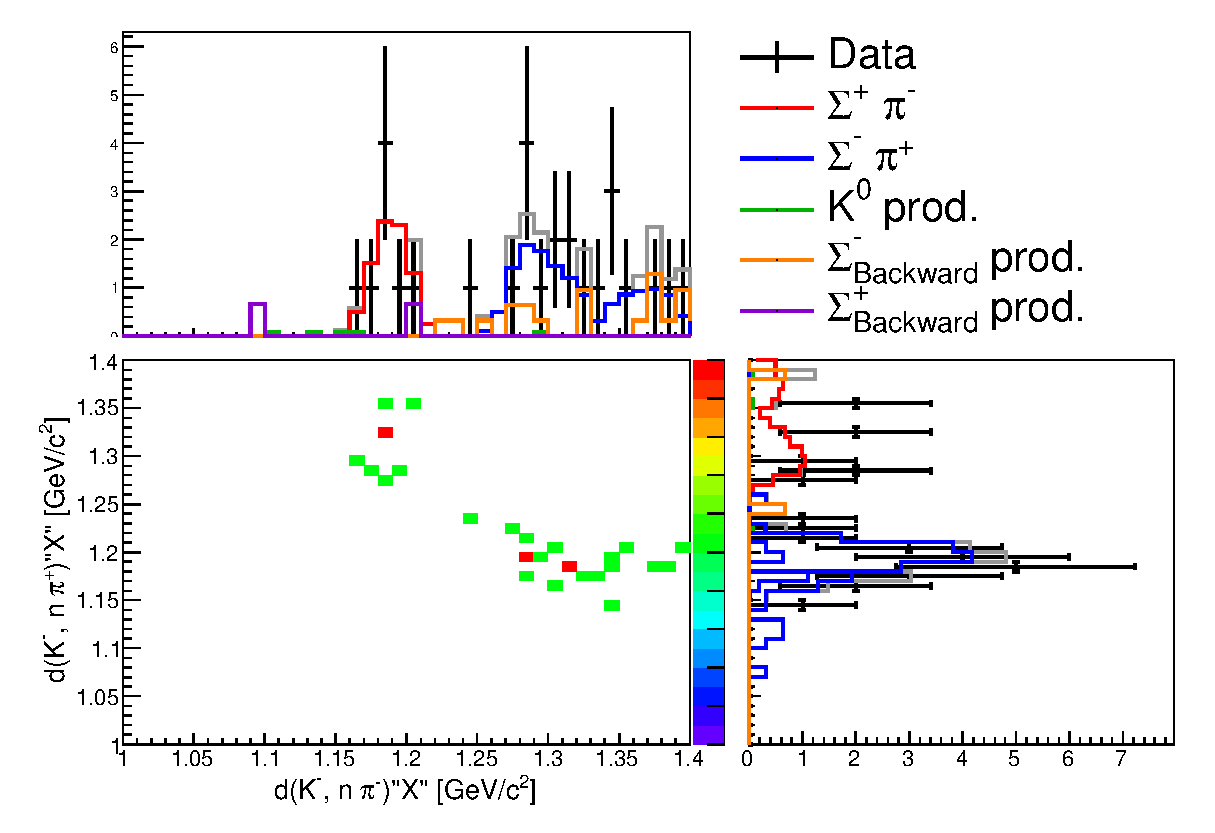
\includegraphics[width=2.2cm]{../pic/Run78/KN_ana_NC170_2sigma/KNpi_MM_24.eps}
    \end{minipage}
  \end{tabular}
  \label{fig:fit_KNpi_MM}
  \caption{
    These figures are presented separately for each bin of $d(K^-, n)$ for fitting to separate $\pi^- \Sigma^+$ and $\pi^+ \Sigma^-$ modes.
    The top left figure shows the lowest missing mass in the $1.35$-$1.36$GeV bin, with the next bin represented as one goes to the right.
    In other words, one row is shown for the 0.05GeV region.
  }
\end{figure}


Next,
we explain the fitting procudure used to separate the $\pi^- \Sigma^+$ and $\pi^+ \Sigma^-$ charge modes of the backward $\pi \Sigma$ scattering,
which serves as the signal in this analysis.
To this end, we use the missing masses of $d(K^-, n \pi^-)$ and $d(K^-, n \pi^+)$,
obtained from events in the $K^-d \rightarrow n \pi^+ \pi^- n$ final state after excluding background contributions
from $K^0$ and $\Sigma^{\pm}_{forward}$ production, as shown in Figure \ref{fig:fit_KNpi_MM_all}.
The lower left panel shows a two-dimensional plot of $d(K^-, n \pi^+)$ versus $d(K^-, n \pi^-)$
while the top and left panels display the one-dimensional spectra of the respective projections
These one-dimensional spectra were used for the fitting.
This figure represents the summed fitting results over all bins of $d(K^-, n)\pi \Sigma$,
and the individual figures for each bin are presented in Figure \ref{fig:fit_KNpi_MM}.
The notations in the figure are consistent with those used for background fitting (Figure \ref{fig:fit_IM}).

The background, represented by the green, purple, and orange lines, is removed within the $3\sigma$ region,
resulting in minimal leakage, although it is still accounted for.
The signal, such as the red line indicating the $\pi^- \Sigma^+$ mode, creates a peak in the $d(K^-, n \pi^-)$ missing mass (top panel)
consistent with the missing $\Sigma$,
whereas the $d(K^-, n \pi^+)$ missing mass (right panel) for the opposite charge does not form a peak but rather shows a broad distribution.
The opposite charge mode, $\pi^+ \Sigma^-$, exhibits similar behavior when the charge is reversed.

The values of $-2\ln(\Lambda)/NDF \sim \chi^2/NDF$ for each bin of $d(K^-, n)\pi \Sigma$ are shown in Figure \ref{fig:tempFit_KNpi_Chi2}.
These fittings yield the $\pi^- \Sigma^+$ and $\pi^+ \Sigma^-$ spectra shown in Figure \ref{fig:piS_num},
which are converted to the double-differential cross section by applying luminosity after acceptance correction,
as described in the next subsection.

\begin{figure}[htbp]
  \centering

  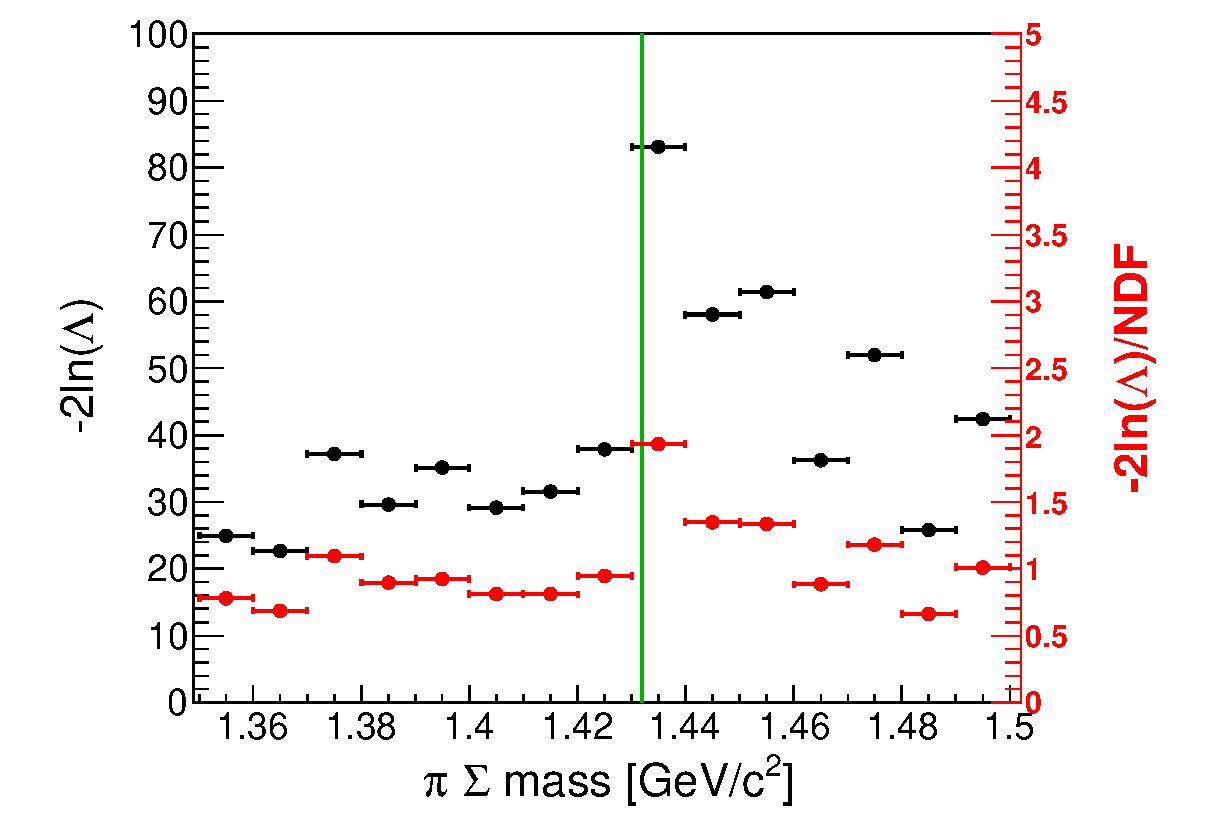
\includegraphics[width=8cm]{../pic/Dron/tempFit_KNpi_MM_Chi2.eps}
  \caption{
    This figure shows the template fitting $-2\log\Lambda$ and $-2\log\Lambda/NDF$ for the separation of $\pi^- \Sigma^+$ and $\pi^+ \Sigma^-$ modes in each $d(K^-, n)$ bin.
    Black and red indicate $-2\log\Lambda$ and $-2\log\Lambda/NDF$, respectively.
    The horizontal axis is represented for $d(K^-, n)$ bins.
  }
  \label{fig:tempFit_KNpi_Chi2}
\end{figure}

\begin{figure}[htbp]
  \centering
  
  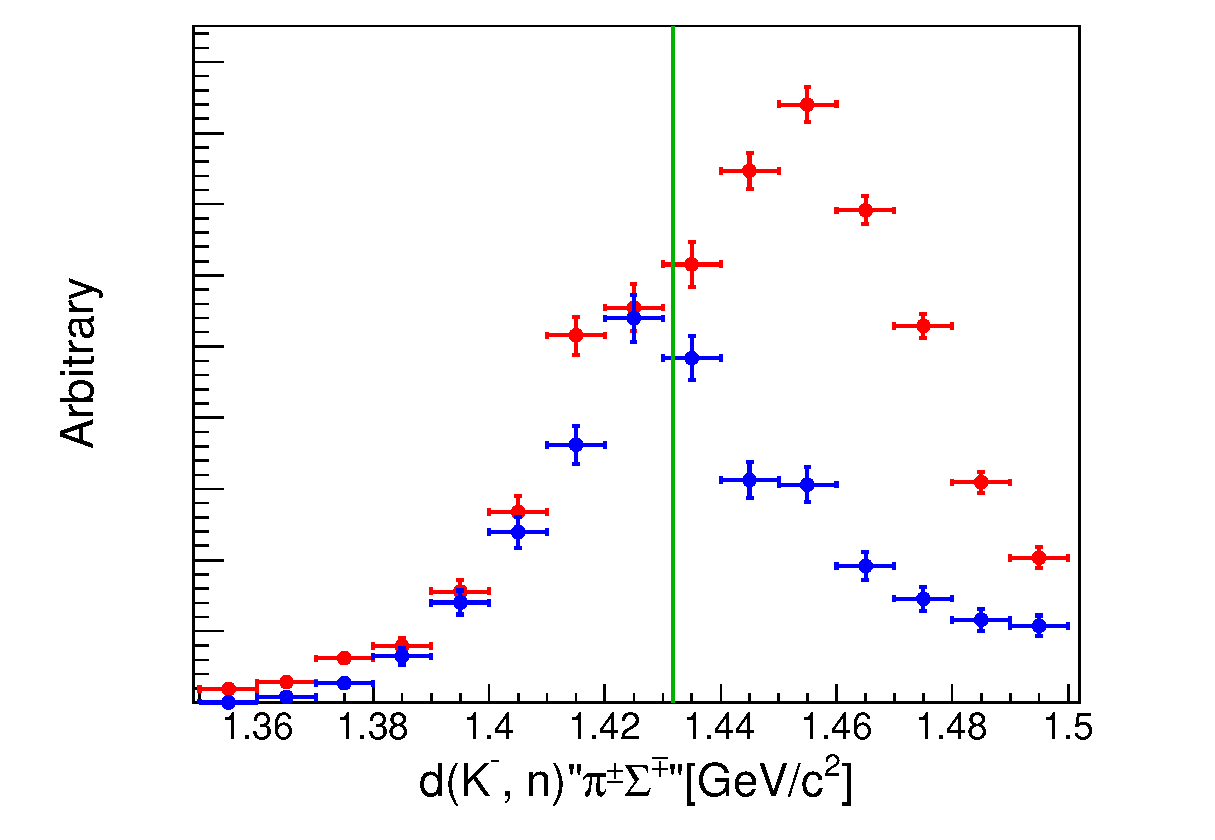
\includegraphics[width=8cm]{../pic/Dron/piS_num.eps}
  \caption{
    The $\pi^-\Sigma^+$ and $\pi^+\Sigma^-$ mode spectra obtained by template fitting are shown in arbitrary units.
    Red and blue lines indicate $\pi^-\Sigma^+$ and $\pi^+\Sigma^-$, respectively.
    The green vertical line is indicated the $\bar{K}N$ threshold.        
  }
  \label{fig:piS_num}
\end{figure}

